% App. D figure: input, listener correction, virtual sensors.
\begin{tikzpicture}[x=1cm,y=1cm]
% ---------------------------------------------------------------- data path
\node[tens=cfN,minimum width=1.35cm,minimum height=1.55cm] (x) at (0,0)
  {$x$\\[1pt]$64\times L'$};
\node[note,below=1pt of x,align=center] {64 canonical channels\\(missing\,=\,0; MEG: 208 sensors)};

\node[nbw={cfN}{1.45}] (V) at (2.45,0.95) {read-out\\$V_m^{\top}$ \,($2\times64$)};
\node[tens=cfN,minimum width=0.7cm] (z) at (4.25,0.95) {$2\times L'$};
\node[nbw={cfN}{1.45}] (U) at (6.0,0.95) {write-back\\$U_m$ \,($64\times2$)};
\node[op=cfN] (plus) at (7.55,0) {$+$};
\draw[ar=cfN] (x.east) -- (plus.west) node[arl,pos=0.52] {identity};
\draw[ar=cfN] ([yshift=0.3cm]x.east) -| ([xshift=-0.35cm]V.west) -- (V.west);
\draw[ar=cfN] (V) -- (z);
\draw[ar=cfN] (z) -- (U);
\draw[ar=cfN] (U.east) -| (plus.north);

\node[tens=cfN,minimum width=1.35cm,minimum height=1.55cm] (xc) at (9.0,0)
  {$\tilde{x}$\\[1pt]$64\times L'$};
\draw[ar=cfN] (plus) -- (xc);
\node[nbw={cfN}{1.6}] (W) at (11.1,0) {virtual sensors\\$1{\times}1$ conv\\$W\!:64\to8$};
\node[tens=cfN,minimum width=0.8cm,minimum height=0.8cm] (v) at (13.05,0) {$8\times L'$};
\draw[ar=cfN] (xc) -- (W);
\draw[ar=cfN] (W) -- (v);
\node[note,right=2pt of v] {to the\\lag-window\\encoder};

% ---------------------------------------------------------------- listener bank
\foreach \i/\d in {2/0.12,1/0.06,0/0} {
  \node[draw=cfN,fill=white,rounded corners=1.5pt,line width=0.5pt,minimum width=3.1cm,
        minimum height=0.55cm] at (4.25+\d,2.35+\d) {};}
\node[font=\scriptsize,align=center] (bank) at (4.25,2.35) {$(U_1,V_1),\dots,(U_M,V_M)$};
\node[note,above=5pt of bank,align=center] {one pair per listener, $2\cdot2\cdot64=256$ parameters;
  $U_m=0$ at initialisation};
\draw[ar=cfX,densely dashed] (bank.south west) ++(0.15,0) -- ([xshift=-0.35cm]V.north)
  node[arl,midway,left] {listener $m$};
\draw[ar=cfX,densely dashed] (bank.south east) ++(-0.15,0) -- ([xshift=0.35cm]U.north);

% ---------------------------------------------------------------- equation
\node[font=\scriptsize,text=cfInk] at (6.0,-1.05)
  {$\tilde{x}=x+U_m V_m^{\top}x$: shared model plus a rank-2,
   listener-specific correction};

% ---------------------------------------------------------------- learned maps
\node[inner sep=0,anchor=north] (lc) at (4.25,-1.45)
  {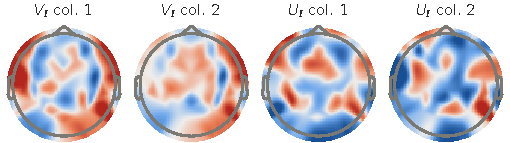
\includegraphics[width=5.2cm]{figures/net_lc_topo.pdf}};
\node[note,below=0pt of lc,align=center] {learned $V_m$ (what the correction reads)
  and $U_m$ (where it writes),\\ KU Leuven listener with the largest correction};
\node[inner sep=0,anchor=north] (vs) at (11.4,-1.45)
  {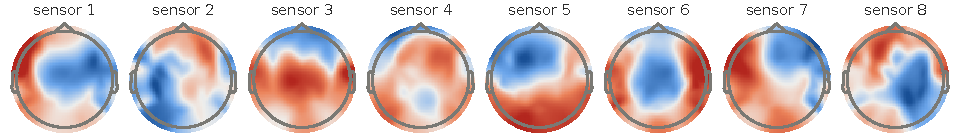
\includegraphics[width=7.1cm]{figures/net_vs_topo.pdf}};
\node[note,below=0pt of vs,align=center] {activation patterns of the 8 virtual sensors
  \citep{haufe2014interpretation}, KU Leuven fold 0};
\end{tikzpicture}
